%!TEX root = ../thesis.tex
%*******************************************************************************
%*********************************** First Chapter *****************************
%*******************************************************************************

\chapter{Background}  %Title of the First Chapter


\section[Introduction]{Introduction}

Neuromorphic computing aims to bridge the gap between neuroscience and artificial intelligence by emulating the structural and functional principles of biological neural systems. At the heart of this vision is a pressing research question: how can we implement biorealistic learning on memristive networks to develop energy-efficient, scalable and adaptive computing architectures? Addressing this question requires a multidisciplinary approach, combining insights from neurobiology, electronic materials science and computational modelling. \\

\noindent Traditional von Neumann architectures \cite{von1993first}, characterised by their separation of memory and processing units, struggle to efficiently handle tasks that the human brain performs effortlessly, such as pattern recognition, sensory integration, and decision making. In contrast, the brain achieves these feats with remarkable energy efficiency and adaptability, in part due to the tightly coupled nature of computation and memory in its neural circuits. Mimicking these biological characteristics in silicon and emerging nanotechnologies has become the guiding principle of neuromorphic engineering \cite{saighi2015plasticity}. \\

\noindent Recent advances in memristive technologies have reignited interest in neuromorphic computing. Memristors, or memory resistors, are two-terminal non-volatile devices that can emulate synaptic plasticity by adjusting their conductance based on the history of voltage and current applied. This property lend itself to naturally support learning rules such as Hebbian learning \cite{hebb2005organization} and spike-timing-dependent plasticity (STDP) \cite{markram1997regulation}. When arranged in crossbar arrays, memristors offer a promising platform for in-memory computation, which can significantly reduce the power and latency associated with traditional data transfer bottlenecks. \\

\noindent This chapter presents a comprehensive discussion of biorealistic learning mechanisms and their physical realisation on memristive networks. By grounding the discussion in the neuroscientific principles that underlie learning and cognition, the chapter aims to elucidate how these biological processes can be abstracted and implemented in hardware. \\

\noindent The chapter begins with an overview of the biological basis of computation, providing an essential neuroscience primer. It then moves to device-level considerations, discussing the properties of memristive devices and their integration into neuromorphic architectures. Throughout, the emphasis is on aligning computational models with biological fidelity, while navigating the constraints and opportunities offered by emerging nanotechnologies.

\section[Neuroscience Primers]{Neuroscience Primers}

Computational neuroscience employs a computational methodology to elucidate the mechanisms underlying brain function. This entails not only identifying the computations performed by the brain but also understanding the interactions between brain elements, such as neurons and synapses, that facilitate these computations.\\

% \noindent The field of computational neuroscience has traditionally adopted a bottom-up approach, commencing with the study of individual neurons and subsequently examining how these can be integrated into progressively larger networks, ultimately leading to the emergence of meaningful behaviour. \\

% \noindent In contrast, psychology and cognitive science have adopted a more top-down approach, commencing with the observation of animal behaviour and subsequently attempting to elucidate the brain mechanisms underlying these behaviours in terms of the higher-level functions of large brain areas. \\

% \noindent This distinction has resulted in a historical focus on developing comprehensive mathematical models of individual neurons and small- to medium-sized networks in computational neuroscience. Recently, however, there has been a convergence with other fields, leading to the creation of neurally detailed models capable of reproducing organism-level behaviors. \\

\noindent This section provides foundational relevant biological details, both at the neural level and at the network level. It should be noted that the models detailed in this dissertaion are still relatively basic in comparison to the extensive body of evidence documenting the neural system \cite{kandel2000principles} which provide the majority of our neural data about these areas. Consequently, this section presents only the most fundamental biological facts relevant to this work.\\

\subsection[Neuron Anatomy and Electrophysiology]{Neuron Anatomy and Electrophysiology}

\noindent  A neuron is a specialised biological cell that processes and transmits information through electrical and chemical signals \cite{mel1994information}. They represent only one of the numerous cell types within the brain, yet they are the most frequently discussed due to their status as the primary computational entities. Their fundamental function is relatively straightforward: neurons receive input from other neurons, and if that input is sufficiently stimulating, they will fire an action potential (also known as a spike), which propagates to other neurons.\\

\noindent Figure \ref{fig:1a} illustrates the basic structure of a neuron. Neurons can be subdivided into three principal parts: the dendrites, the cell body (soma), and the axon. Neurons receive input currents via their dendrites, which then transmit or channel this into the cell body, called the soma. When a neuron spikes, it sends current down its axon, which results in the release of neurotransmitter(s) at the synapses. These are connections from a neuron's axon to the dendrites of other neurons, and the neurotransmitter release causes dendritic input currents in these other connected neurons. \\

\begin{figure}[htbp!] 
    \centering    
    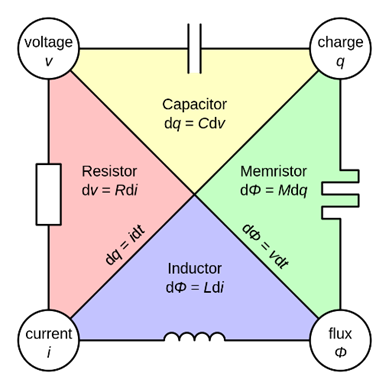
\includegraphics[width=0.5\textwidth]{Chapter1/Figs/1a.png}
    \caption[Labeled diagram of the neuron.]{Labeled diagram of the neuron, nerve cell that is the main part of the nervous system. A neuron's dendrites include synapses that allow it to accept input from other neurons. The dendrites carry current to the soma, which is where electrical charge is integrated. If the neuron membrane gets sufficiently polarised, an action potential (also known as a spike) travels down the axon. This causes neurotransmitters to be released at synapses, resulting in currents in the dendrites of postsynaptic neurons.}
    \label{fig:1a}
    \end{figure}

\noindent From a computational perspective, the soma represents the integration point for all incoming currents from dendrites \cite{polsky2004computational}, marking the initiation of the action potential generation process (Figure \ref{fig:1b}). When a neuron is at rest, the soma exhibits a negative charge. This is referred to as the resting voltage and is maintained by ion pumps that regulate the concentration of ions (predominantly sodium, $Na^+$, potassium, $K^+$, and calcium, $Ca^{+2}$) within the cell. \\


\noindent As the currents arrive from the dendrites, they initiate a process of depolarisation of the cell \cite{johnston1996active}. Once the voltage within the soma reaches a sufficient level, it initiates the opening of voltage-activated sodium channels, which permit the influx of sodium ions into the cell, further depolarising it. This process persists until the electrical gradient resulting from the accumulation of sodium ions reaches a point where it is no longer in equilibrium with the chemical gradient caused by the imbalance of sodium within and outside the cell. This leads to a notable increase in the neuron's positive charge, exceeding the resting voltage. \\

\noindent Furthermore, this substantial depolarisation also activates voltage-gated potassium channels, which subsequently permit the release of potassium ions from the cell, thereby facilitating repolarisation. Concurrently, the sodium channels undergo inactivation. The opening of potassium channels ultimately results in the cell reaching a voltage below its resting level, a state known as hyperpolarisation. The sodium channels remain inactivated and the potassium channels remain open for a period of time following the spike. \\

\begin{figure}[htbp!] 
    \centering    
    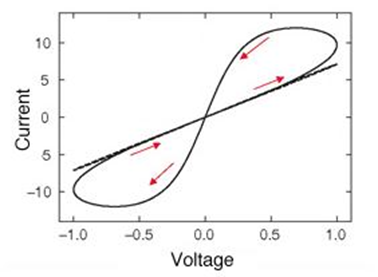
\includegraphics[width=0.45\textwidth]{Chapter1/Figs/1b.png}
    \caption[Spiking dynamics of a neuron.]{The action potential and the underlying conductance and currents with respect to time \cite{squire2012fundamental}. It should be noted that the increased conductance for $Na^+$ (and its inward flow) is associated with the rising phase of the action potential, whereas the slower increase in conductance for $K^+$ (and its outward flow) is associated with repolarisation of the membrane and with afterhyperpolarisation. The reduction in $I_{Na}$ before the peak of the action potential (even though $G_{Na}$ is still high) is due to inactivation of the Na+ channels.}
    \label{fig:1b}
\end{figure}

\noindent The combination of these factors renders it almost impossible for the neuron to fire during this time; this is referred to as the absolute refractory period. The change in ionic concentrations within the cell is relatively minor during a single spike, but over the course of numerous spikes, the ion pumps are required to maintain the optimal concentrations of sodium and potassium. Other currents, most notably calcium currents, are present in some neurons. \\

\noindent The rapid depolarisation associated with an action potential not only causes an increase in the somatic voltage potential, but also results in partial depolarisation of the axon segments situated in closer proximity to the soma. This results in the opening of sodium channels in that part of the axon, which in turn causes further depolarisation and the opening of sodium channels in the subsequent section of the axon. In this way, the somatic spike triggers a voltage wave that travels down the axon, eventually leading to the release of neurotransmitter(s) from synaptic vesicles situated near the ends of the axon. \\

% \noindent Axons are responsible for transmitting long-range signals in the brain, and thus exhibit considerable variation in length, contingent on whether a given neuron is connected to neighbouring neurons or to neurons situated in a different brain region. To facilitate long-range transmission, axons are coated in myelin, a substance composed mainly of lipids and thus a good electrical insulator.\\

% \noindent This enables the propagation of current down the axon. The high proportion of fat makes myelin white; bundles of axons are responsible for the "white matter" parts of the brain. In contrast, the "grey matter" is composed mainly of neuron dendrites, somas, and short-range axons.\\

% \noindent Dendrites are thin processes that extend away from the soma to connect to the axons of other neurons \cite{johnston1996active}. They serve to transmit current from synapses with other neurons to the soma. Initially, it was thought that they only conducted current passively; however, research has demonstrated that they possess active conductance mechanisms that are analogous to those involved in spike generation and propagation down an axon.\\

% \noindent Dendrites are also traditionally considered to act in a linear manner, whereby inputs from numerous synapses are accumulated over time and space. This remains a prevalent assumption in numerous computational models. However, recent studies have demonstrated that the summation of signals in dendrites is more intricate, exhibiting a combination of linear and nonlinear (sigmoidal) elements.\\

% \noindent Neurons are connected to one another by synapses, which facilitate the connection between the axon of the presynaptic neuron and a dendrite of the postsynaptic neuron. Upon the occurrence of a spike in the presynaptic neuron, an electrical pulse is transmitted along the axon, reaching the presynaptic terminals of all synapses situated along its length. The synaptic vesicles, which are filled with neurotransmitter, are located at the terminals. \\

% \noindent When an electrical pulse is generated, it causes the vesicles to release neurotransmitter into the synaptic cleft, which is the narrow space between the presynaptic terminal and the postsynaptic terminal. This neurotransmitter then activates receptors on the postsynaptic terminal, which open and permit the flow of current into the postsynaptic cell. The specific neurotransmitter utilized by the synapse is contingent upon the presynaptic neuron. \\

\noindent All synapses on a neuron's axon release the same neurotransmitter or combination of neurotransmitters, a phenomenon known as Dale's principle. At the time of its development, Dale's principle was based on the assumption that each neuron produced a single type of neurotransmitter. However, evidence of cotransmission was only discovered later \cite{burnstock2004cotransmission}, with the understanding that neurotransmitters can be excitatory or inhibitory. It is not the case that any neurons play both an excitatory and inhibitory role with respect to different postsynaptic cells.

\subsection[Spiking Neuron Dynamics]{Spiking Neuron Dynamics}

\noindent In recent times, the number of available neuron models has proliferated. The models currently in use in the literature range from the simplest possible rate-neuron model, namely binary threshold units \cite{stocks2001information}, to complex multi-compartmental models that account for detailed dendritic morphologies \cite{markram2015reconstruction}. In the context of large-scale neural models aiming to reproduce high-level behaviours, single-compartment neuron models remain the prevailing approach. \\

\noindent These models treat the neuron as a single electrical compartment, combining the dendrites, soma, and axon. In contrast, multi-compartmental models represent the neuron as comprising multiple electrical compartments, with equations that describe the influence of activity in one compartment on that of another. By modelling the spike separately from the rest of the neural dynamics, it is possible to separate time scales, thereby avoiding the need for additional computational resources to model the spike trajectory \cite{abbott1999lapicque}. \\

% \noindent The number of compartments in a model can vary considerably, from a minimalistic two-compartment structure, typically comprising one for the dendrites and one for the soma, to a more elaborate configuration comprising thousands of compartments. \\

% \noindent The number of compartments in a model is directly proportional to the amount of computing power required for simulation and the complexity of the resulting behaviour. For these reasons, models that seek to reproduce behaviour predominantly utilise either single-compartment neurons or simpler models that do not model the electrical activity of the neuron at all. \\

% \noindent Single-compartmental neuron models can be classified according to two key dichotomies: firstly, the rate-based versus spike-based dichotomy; and secondly, the static versus dynamic dichotomy. The distinction between rate-based and spiking neuron models concerns the nature of the output: is it a continuous value, represented by a firing rate, or a discrete value, represented by a spike.\\

% \noindent The distinction between static and dynamic models concerns the extent to which the model exhibits internal dynamics. In a static model, the output at a given point in time is independent of the neuron's past history and solely contingent on its instantaneous input. In contrast, a dynamic model allows for some degree of dependence on the neuron's past trajectory.\\

% \noindent Dynamic neuron models possess a state, which is to say, internal variables that evolve over time and are not directly computable from the present input to the model. They are typically expressed using differential equations. In contrast, static models output a function of the current input only; thus, they do not require differential equations to express them. \\

% \noindent It is important to note that the distinction between static and dynamic neurons does not necessarily refer to whether the neuron is being used as a static nonlinearity, evaluated at a single point in time on an input value, or as a dynamic nonlinearity, evaluated over a period of time on an input signal. \\

% \noindent Static neurons can be evaluated dynamically by evaluating them independently at each successive point in time on the input value. In contrast, there is no general method for evaluating dynamic neurons statically, as their input at any given point in time is contingent upon their internal state, which is a dynamic process that evolves over time. \\

% \noindent In some cases, it is possible to determine a firing rate response curve, also known as an I-F response curve or rate response function, for dynamic neuron models. This curve maps every constant value of the input current to a constant firing rate output. This can be determined analytically or empirically by applying a constant input current and measuring the rate of the output spikes, this can even be done in real neurons in vitro. \\

% \noindent However, many neuron models will not output spikes at a constant rate, even for a constant input, due to changing internal dynamics. In such cases, the rate-response function only captures part of the model, and will be different depending on the state of the model and how it is measured or calculated. \\

% \begin{table}[]
% \caption{Neuron Model Dichotomies.}
% \centering
% \begin{tabular}{|c|c|c|}
% \hline
%                  & \textbf{Rate}                                                                  & \textbf{Spiking}                                             \\ \hline
% \textbf{Static}  & Sigmoid Rate LIF                                                               & Poisson Spiking                                              \\ \hline
% \textbf{Dynamic} & \begin{tabular}[c]{@{}c@{}}Adaptive Rate LIF\\ Sigmoid with State\end{tabular} & \begin{tabular}[c]{@{}c@{}}Hodgkin-Huxley\\ LIF\end{tabular} \\ \hline
% \end{tabular}
% \label{table:4a}
% \end{table}

% \noindent Table \ref{table:4a} illustrates the manner in which a small selection of neuron models align with these dichotomies. In the static rate category, the models in question take in a continuous value and output a continuous function of that value. This encompasses the majority of non-linearities employed in machine learning (such as sigmoids or rectified linear units), in addition to the analytic firing rate for the LIF neuron model. \\

% \noindent In the static spiking category, models are characterised by the output of a discrete (binary) function of their continuous input. This category is primarily composed of Poisson-spiking neurons, which fire probabilistically based on their instantaneous firing rate. This implies that the probability of firing at a given time is independent of past firings. Furthermore, Poisson spiking can be applied to a dynamic rate model, whereby the probability of spiking is independent, but the spike rate is a dynamic process. \\

% \noindent Dynamic rate models possess an internal state that influences their continuous output, in addition to the input. This encompasses the analytic LIF rate model with adaptation, which possesses an intrinsic adaptation parameter that increases when the neuron is active and discounts the firing rate. Furthermore, the category encompasses sigmoid neuron models that possess an underlying voltage that is dynamically correlated with the neuron inputs \cite{lillicrap2016random}. \\ 

% \noindent The dynamic spiking category also includes the LIF neuron model, the Hodgkin-Huxley model, and more intricate multi-compartmental models. Within the category of spiking models, a distinction can be made between those that output instantaneous spikes (e.g., LIF) and those that output spikes that vary across time (e.g., Hodgkin-Huxley). Recently, another study have employed such models in the context of deep networks \cite{guerguiev2017towards}, subject to biological constraints. \\

% \noindent Another potential distinction can be made between models that output stereotyped spikes, where the size of each spike is identical, and those that output variable-sized spikes. Models of cortical neurons that output instantaneous spikes (e.g., LIF) almost invariably output stereotyped spikes. This is due to the fact that spikes in cortical neurons are almost identical in terms of magnitude, duration, and shape.\\

% \noindent It is widely believed that none of these factors carry information. Even among models that have spikes that vary across time (e.g., Hodgkin-Huxley), the spike magnitude, duration, and shape are quite consistent between spikes. Therefore, the majority of spiking cortical neuron models exhibit stereotyped spikes. \\

% \noindent By modelling the spike separately from the rest of the neural dynamics, it is possible to separate time scales, thereby avoiding the need for additional computational resources to model the spike trajectory, which is characterised by stereotyped details of little interest \cite{abbott1999lapicque}. \\

\begin{figure}[htbp!] 
    \centering    
    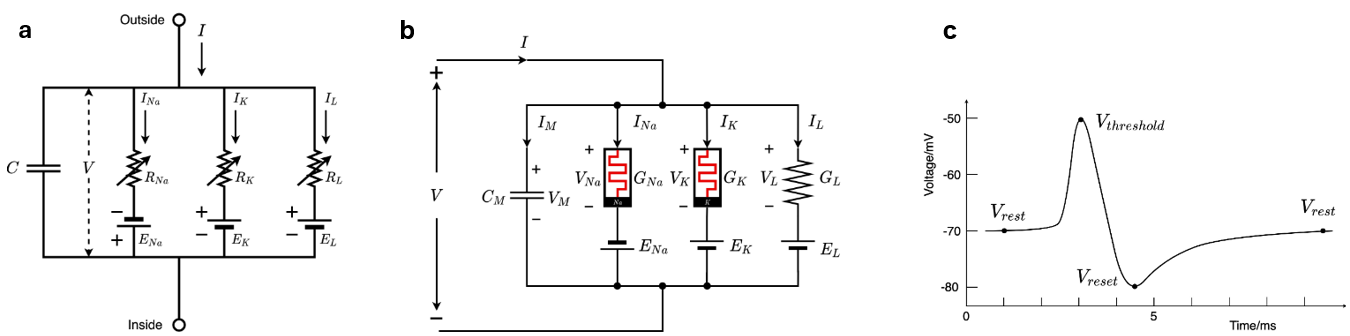
\includegraphics[width=1\textwidth]{Chapter1/Figs/1c.png}
    \caption[Hodgkin-Huxley neuron model.]{Hodgkin-Huxley neuron model. (a) An equivalent circuit for the HH models \cite{hodgkin1952quantitative}. (b) An equivalent circuit for memristive HH model \cite{chua2012hodgkin}. (c) An action potential waveform, which demonstrates the resting, threshold, and reset potentials. }
    \label{fig:1c}
\end{figure}

\noindent A significant proportion of the most influential findings in computational neuroscience are based on mathematically detailed models of neuronal functioning. One of the most renowned of these is the Hodgkin-Huxley model of the squid giant axon \cite{hodgkin1952quantitative}. the Hodgkin–Huxley (HH) model is one of the most widely used, comprising a set of nonlinear differential equations that accurately approximate the electrical signals of neurons \cite{chua2012hodgkin}. \\

\noindent Figure \ref{fig:1c}(a) depicts the HH neural model, wherein the time-varying nonlinear conductor $R_{Na}(GNa)$ and $R_K(G_K)$ represent the sodium and potassium channels, respectively, while the linear conductor $R_L(G_L)$ simulates leak channels and $C$ models the membrane of a neuron. The equations of the HH model are presented below: 
\begin{align}
    C \frac{dV_m(t)}{dt} = I_C(t) + \sum_{k}^{}I_k(t) \label{eq:1.1} 
\end{align}

\noindent In this context, $V_m$ represents the membrane potential. $\sum_{k}^{}I_k(t)$ denotes the sum of the ionic currents flowing into the neuron. This can be formulated by three ion currents, as follows:
\begin{align}
    \sum_{k}^{}I_k &= C_m \frac{dV_m}{dt} + G_Kn^4(V_m - V_K) + G_{Na}m^3(V_m - V_{Na}) + G_L (V_m - V_L) \label{eq:1.2} \\
    \frac{dn}{dt} &= \alpha_n(V_m)(1-n)-\beta_n(V_m)n \label{eq:1.3} \\
    \frac{dm}{dt} &= \alpha_m(V_m)(1-m) - \beta_m(V_m)m \label{eq:1.4} \\
    \frac{dh}{dt} &= \alpha_h(V_m)(1-h)-\beta_h(V_m)h \label{eq:1.5}
\end{align}

\noindent The reversal potentials $V_K$, $V_{Na}$, and $V_L$ are the three parameters in question. The rate constants $\alpha_i$ and $\beta_i$, which depend on the membrane potential, describe the behaviour of the $i^{th}$ ion channel. The maximal value of the conductance is represented by $G_K$, $G_{Na}$, and $G_L$. Finally, the dimensionless quantities \textit{n}, \textit{m}, and \textit{h}, which lie between 0 and 1, are associated with three ion channels. \\

\noindent In order to achieve the optimal fit for human cardiac action potentials, the HH model is reduced by setting the leakage channel conductance to $G_L = 0$  \cite{noble1962modification}.It has been demonstrated that $G_{Na}$ and $G_K$ are memristors \cite{chua1976memristive}, as illustrated by the equivalent circuit in figure \ref{fig:3c}(b). \\

\noindent The integrate-and-fire (IF) neuron \cite{lapicque1907louis} constituted one of the earliest computational models of a neuron. This model was developed prior to the ability of researchers to measure the electrical and chemical changes occurring in a functioning neuron. It is based on the premise that the neuron membrane can be modelled as a capacitor that stores charge over time \cite{abbott1999lapicque}.\\

\noindent As the name suggests, the IF model exhibits two principal behaviours: The model integrates current over time, as would be expected of a capacitor, and fires when the voltage reaches a threshold. Furthermore, the model may or may not incorporate a leak term, which represents a resistor in parallel with the capacitor that permits the dissipation of charge over time. The model with a leak term is typically designated as the leaky integrate-and-fire (LIF) model. While the term "integrate-and-fire (IF) model" can be used interchangably. \\

\noindent With the objective is to identify how the neuron's membrane voltage evolves over time and, based on this, to determine when the neuron spikes. The charge \textit{Q} across a capacitor is given by $Q = V \times C$, where \textit{V} is the voltage across the capacitor and \textit{C} is the capacitance. Differentiating this with respect to time, we find that the membrane voltage $\textit{V(t)}$ of the neuron is governed by:
\begin{align}
    C \frac{dV(t)}{dt} = J(t) \label{eq:1.6} 
\end{align}

\noindent In this context, \textit{J(t)} represents the input current to the neuron over time, whereas \textit{C} denotes the membrane capacitance. The current here is the time derivative of charge. Equation \ref{eq:1.6} demonstrates that the IF neuron simply integrates the input current over time. It is still necessary to identify the point at which the neuron spikes. \\

\noindent This is achieved by defining a threshold voltage, $V_{th}$, which is exceeded when the voltage passes this threshold, resulting in the neuron firing. This is a fundamental principle in neurophysiology: once the neuron voltage passes a threshold, the neuron begins firing a spike, and once this firing process begins, it is almost impossible to reverse. \\

\noindent A reset procedure is finally defined. Once a neuron has fired a spike, the membrane voltage is reset to the resting potential, $V_{rest}$. This phenomenon can be attributed to physiological processes. Following the occurrence of a spike in a neuron, other ionic currents, typically potassium, are initiated, leading to a restoration of the membrane voltage towards the resting potential.\\

% \noindent Some integrate-and-fire models may also incorporate an absolute refractory period, defined as a time interval during which the voltage is maintained at the resting potential $V_{rest}$ following a spike. In cortical neurons, post-spike potassium currents are sufficiently strong to prevent another spike from occurring for a considerable duration. This time interval is referred to as the absolute refractory period. The model accounts for this by holding the membrane voltage at $V_{rest}$ for a duration equal to the absolute refractory period. \\

\noindent The leaky integrate-and-fire (LIF) model \cite{knight1972dynamics} incorporates an additional physiological factor: Neuron membranes are not perfect capacitors; rather, they slowly leak current over time, pulling the membrane voltage back to its resting potential. Therefore, the membrane is modelled as a capacitor and resistor in parallel, which allows for the neuron to exhibit a degree of "forgetting": in the absence of any input, the membrane voltage will return to its resting potential \cite{koch2004biophysics}. The LIF dynamics are captured by the following equation:

\begin{align}
C \frac{dV(t)}{dt} = J(t) - \frac{1}{R} (V - V_{rest}) \label{eq:1.7} 
\end{align}

\noindent In this model, \textit{R} represents the membrane resistance, and the remaining parameters are consistent with those of the IF model. The resetting procedure is also identical to that of the IF model.\\

\noindent The LIF model comprises a number of parameters, including $C, R, V_{rest}$ and $V_{th}$. It is possible to normalise the model in order to reduce the number of parameters while maintaining the full dynamics of the original model. In particular, the model can be manipulated so that the normalised voltage lies within the range [0, 1], with a normalised resting potential of zero and a normalised firing threshold of one. Initially, Equation \ref{eq:1.7} is multiplied by R to give:

\begin{align}
    \tau_{rc} \frac{dV}{dt} &= RJ(t) - V + V_{rest} \label{eq:1.8} \\
    \tau_{rc} &= R \times C \label{eq:1.9} \\
    \bar{V} &= \frac{V - V_{rest}}{V_{th} - V_{rest}} \label{eq:1.10} \\
    \bar{V_{rest}} &= \frac{V_{rest}}{V_{th}} \label{eq:1.11} 
\end{align}

\noindent By substituting $\bar{V}$ and $\bar{V_{rest}}$ into equation \ref{eq:1.3} to give:


\begin{align}
    \tau_{RC}(V_{th} - V_{rest})\frac{d\bar{V}}{dt} &= RJ(t) - \bar{V}(V_{th} - V_{rest})
    \label{eq:1.12} \\
    \tau_{rc}\frac{d\bar{V}}{dt} &= \frac{R}{V_{th} - V_{rest}} J(t) - \bar{V} \label{eq:1.13} \\
    \tau_{rc} \frac{d\bar{V}}{dt} &= \bar{J}(t) - \bar{V} \label{eq:1.14} 
\end{align}

\noindent When the firing threshold for the new equation $\bar{V_{th}} = 1$, the voltage resets to $\bar{V_{rest}} = 0$, and $\bar{J}(t) = \frac{R}{V_{th} - V_{rest}} J(t)$. It can be observed that $\bar{J}(t)$ is merely a linear transformation of $J(t)$. Consequently, Equation \ref{eq:1.14} retains the full dynamics of Equation \ref{eq:1.7} for a scaled input, but with only one parameter, $\tau_{RC}$. \\

\noindent It should be noted that both $\bar{V}$ and $\bar{J}$ are unitless quantities. Conventionally, the unitless space is employed exclusively, and the quantities are often referred to simply as \textit{V} and \textit{J}, despite the fact that they are not voltages or currents. This simplifies the mathematical representation, without limiting the generality of the models. \\

\noindent Equation \ref{eq:1.14} provides an exact description of the circumstances under which the model neuron will spike in response to a given input current, \textit{J(t)}. However, in some cases, it is sufficient to consider only the spike rate, that is, the number of spikes per second that the neuron will produce in response to a given input current. \\

\noindent In the case of the LIF model, it is possible to determine the analytical firing rate for a constant input current. This is achieved by calculating the inter-spike interval (ISI), which is the time between one spike and the next. The firing rate is then given by the inverse of the ISI. When a constant input current, $J(t) = j$, is provided, it is possible to solve Equation \ref{eq:1.14} in order to find the neuron voltage over time. 
\begin{align}
    V(t) = (V(0) - j)e^{\frac{-t}{\tau_{rc}}} + j \label{eq:1.15}
\end{align}

\noindent In the absence of spikes, the objective is to ascertain the time required for the voltage to increase from$ V(0) = 0$ to $V(t) = 1$. This property will only occur if $j > 1$. Substitution into Equation \ref{eq:3.15} and subsequent solution for \textit{t} yields:
\begin{align}
    t = - \tau_{RC} log \left( - \frac{1}{j} \right) \label{eq:1.16}
\end{align}

\noindent Incorporating the refractory period and performing the inversion, the spike rate \textit{r} for the LIF neuron is given by:
\begin{align}
    r &= \begin{cases}
    \frac{1}{t_{ref} - \tau_{RC} log \left( 1 - \frac{1}{j} \right)} & \text{ if } j > 1 \\ 
    0 & \text{ otherwise }  
    \end{cases} \label{eq:1.17}
\end{align}


% \noindent For simplicity and hardware tractability, many neuromorphic models use the leaky integrate-and-fire (LIF) model.

\subsection[Synaptic Transmission and Plasticity]{Synaptic Transmission and Plasticity}

